\documentclass[11pt]{article}
\title{Report iteration 2 - SWOP}
\author{Dieter Geboers, Wouter Schaekers, Stefaan Truijen\\ - \\ Professor: Tom Holvoet \\ Project Advisor: Willem Penninckx}
\date{2011-12-31}
\usepackage[pdftex]{graphicx}
\usepackage{fancyhdr}
\usepackage[top=20mm,bottom=20mm,left=20mm,right=20mm]{geometry}
\usepackage{hyperref}
\pagestyle{fancy}
\begin{document}
\maketitle

\section{Introduction}
Let's start off by saying we have the feeling that iteration two went a lot better than iteration one.
\\*After the feedback session of iteration one, Thibault decided to drop out of the course. We were left with only three members. We failed to make the deadline for the report on the testing strategy.
\\*However, we did not let that get to us or let it influence the quality of the report, design and code we made. In fact, we put a maximum amount of effort in doing the assignment as best as we could.\newline

Firstly, we will give you a state of affairs and some numbers about the project. Next, we will discuss the big picture from the current software design we made. We'll specifically elaborate on the Scheduler and everything related to it, seeing as we have put the bigger part of our work in creating a scheduler that is very decent. Then we will list some of the "temporary fixes" we implemented, but that we have planned to be improved due to iteration 3. Finally we'll try to draw a couple of conclusions and give you a brief view on our experience of this iteration.

\pagebreak
\tableofcontents
\pagebreak

\section{State of affairs}
We have managed to successfully create a design of every aspect of the assignment. The implementation is almost done, but not just yet. Due to a lack of time(which was probably induced by the fact we hadn't brought iteration one to an end), we were forced to implement a couple of things in a "dirty" kind of fashion. We, however, will implement our actual design by the deadline of iteration three for the following things:
\begin{enumerate}
\item{The way medication items (vitamins, asprin,...) gets handled is currently by using instanceof. We plan to implement a factory pattern here in the future.}
\item{Machines should also be implemented by using a factory pattern instead of "builders".}
\item{Treatments aswell, will be implemented with a factory pattern.}
\item{UnscheduledTaskTest class contains a lot of seemingly random stuff and will be refactored to something cleaner.}
\item{Documentation may be sloppy, missing or inaccurate for some methods and classes.}
\item{Not all methods have been implemented defensively. This is a very small minority of methods. Contrary to iteration one, most methods and classes are completely defensive.}
\end{enumerate}

%%%%%%%%%%%%%%%%%%%%%%%%%%%%
% Vul de puntjes in, slet! %
%%%%%%%%%%%%%%%%%%%%%%%%%%%%

Currently the total amount of lines is nearing 20,000 which is enough for a grand total of ... classes! Of those 20,000 lines, Eclemma tells us that ... \% is covered. About 3,500 lines of those are in UI. We opted not to test UI with unit tests as the results depend on user input, which is harder than just running them and seeing where it goes wrong, knowing that the underlying system should be monkey proof after extensive unit testing.

We have spent about ... hours averagely per person on this iteration. You can find the total amount of working hours for each person in the table below.
\begin{center}
    \begin{tabular}{ | l | l | l | p{10cm} |}
    \hline
    Dieter & Stefaan & Wouter\\ \hline
    1337 & 9001 & SO MANY HOURS\\
    \hline
    \end{tabular}
\end{center}
For an even more detailed log of the working hours (containing dates and more information about who was present and what happened at what time), we would like to refer to \url{http://code.google.com/p/swop-dswx/wiki/WorkingHours} .

\section{The design}
In this chapter we will inform you about the design we've made and will elaborate on some of choices we have made. Firstly, we have modeled our system in 3 layers. 
\begin{itemize}
\item{User interface layer}
\item{Controller layer}
\item{System layer}
\end{itemize}
All communication from the user with the system has to pass through the layer of controllers (same goes the other way around) to assure that our system does what it is supposed to without getting in an inconsistent state.
\\On the next four pages you will find a class diagram of the system layer of our program. We find this to be the most interesting layer as the controller layer is fairly analogous to what controllers normally look like and as talking about the user interface layer will not inform the reader about what he/she probably would like to know. In order to read the class diagram as it was originally constructed, we would advise you to put the pages next to eachother from left to right. As big class diagrams tend to not be legible, we'd like to refer to an online version of this diagram just in case: \url{http://www.student.kuleuven.be/~s0214045/class%20diagram.png} .\\

\subsection{Patientfilemanager, patientfile, diagnose, treatment}
We had a question about where we should store what treament is associated with what diagnosis. In our eyes, there were two possible solutions.
\subsubsection{Solution}
\underline{Description}: We give PatientFile a field that is a collection of all Diagnosis ever made for this patientfile. Also Diagnosis gets a field that is a collection of all Treatments that have been made for this diagnosis.

\underline{Pro}: Low coupling, high cohesion and information expert for PatientFile are in good shape. PatientFile only has one dependency and does not need to manage treatments on its own.

\underline{Contra}: There will be a deep level of function calls if a list of Treatments is needed: from the controller level all the way over to the Treatment level.
\begin{center}
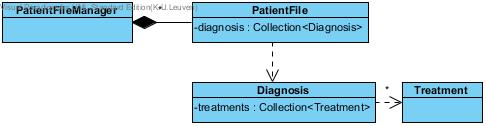
\includegraphics[width=130mm, height=27mm]{patientfilediagwin.jpg}
\end{center}
After a meeting with our project advisor, we noticed that in this solution, the GRASP patterns weren’t violated and the design is arguably elegant. That is why we opted to go with this solution.
\subsubsection{Alternative solution}
\underline{Description}: We keep a map from Diagnose to Treatment in PatientFile.

\underline{Pro}: Easy and efficient access to Treatments.

\underline{Contra}: Gives the patientfile too much responsibility. Also violates the information expert GRASP pattern. 
\begin{center}
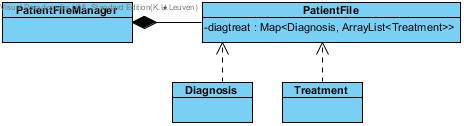
\includegraphics[width=130mm, height=27mm]{patientfilediagfail.jpg}
\end{center}
As stated above, we did not chose to implement this solution after noticing that it violated information expert.\\
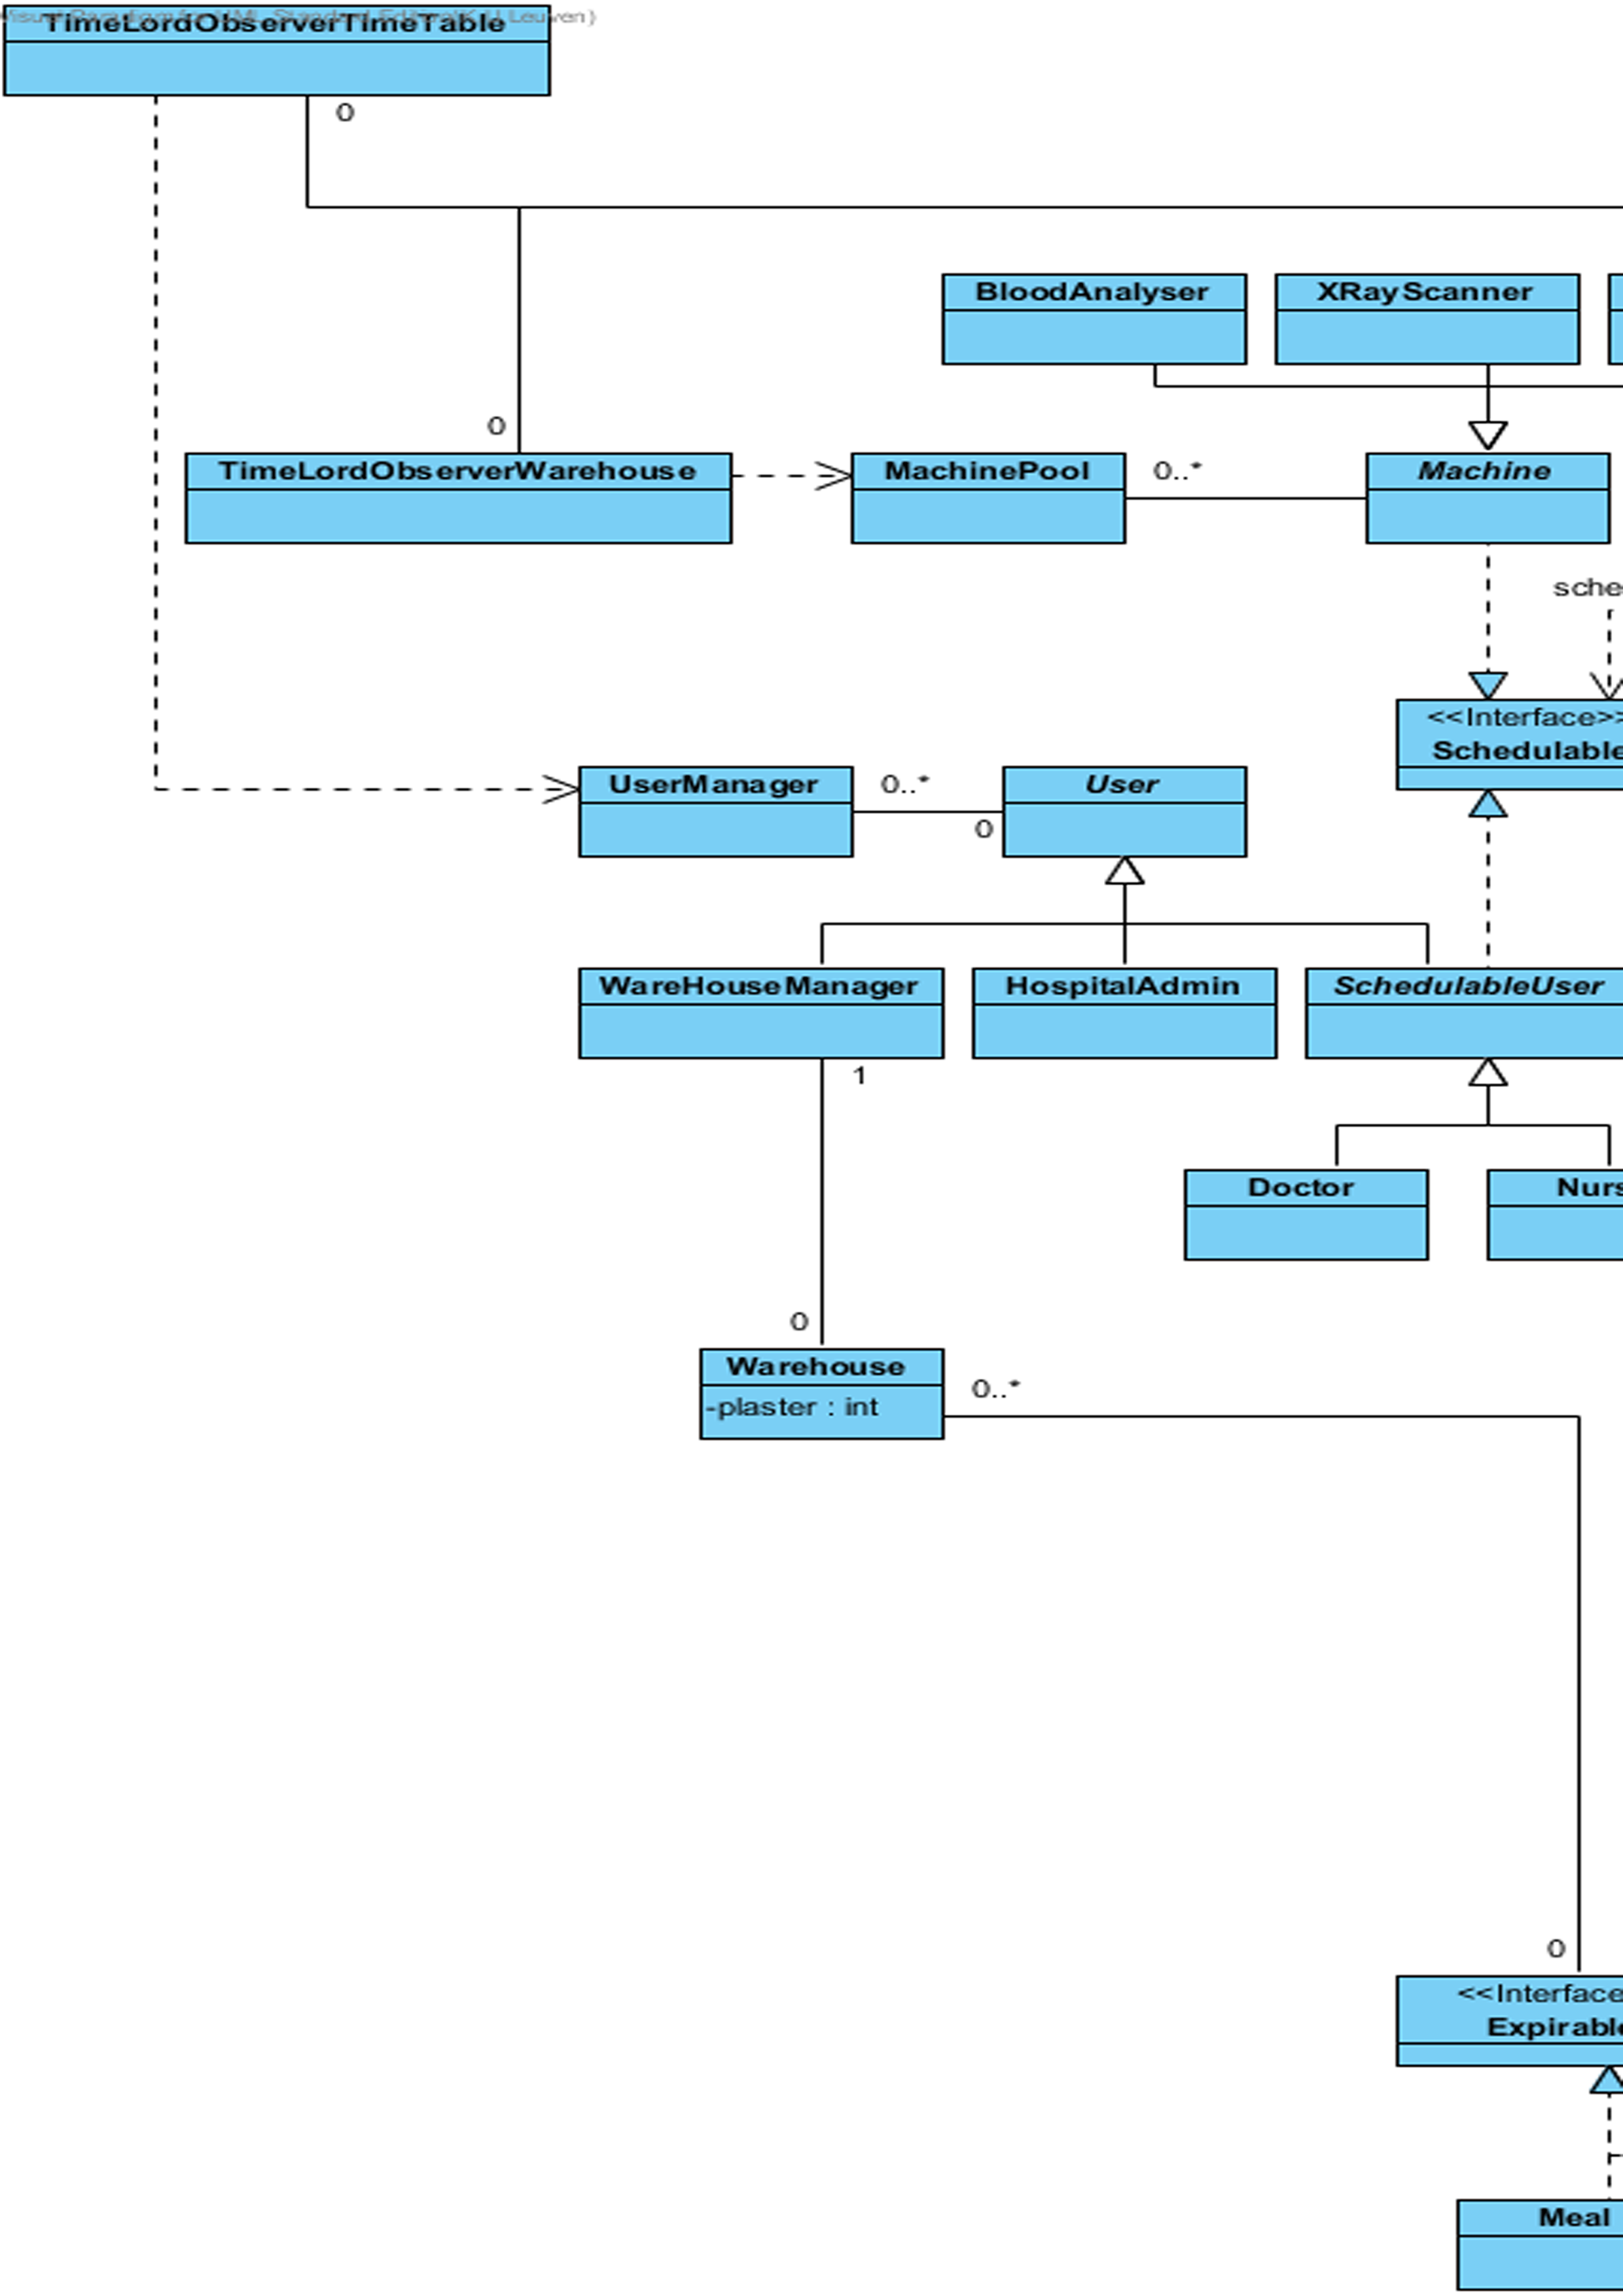
\includegraphics[width=170mm]{left1.png}\\
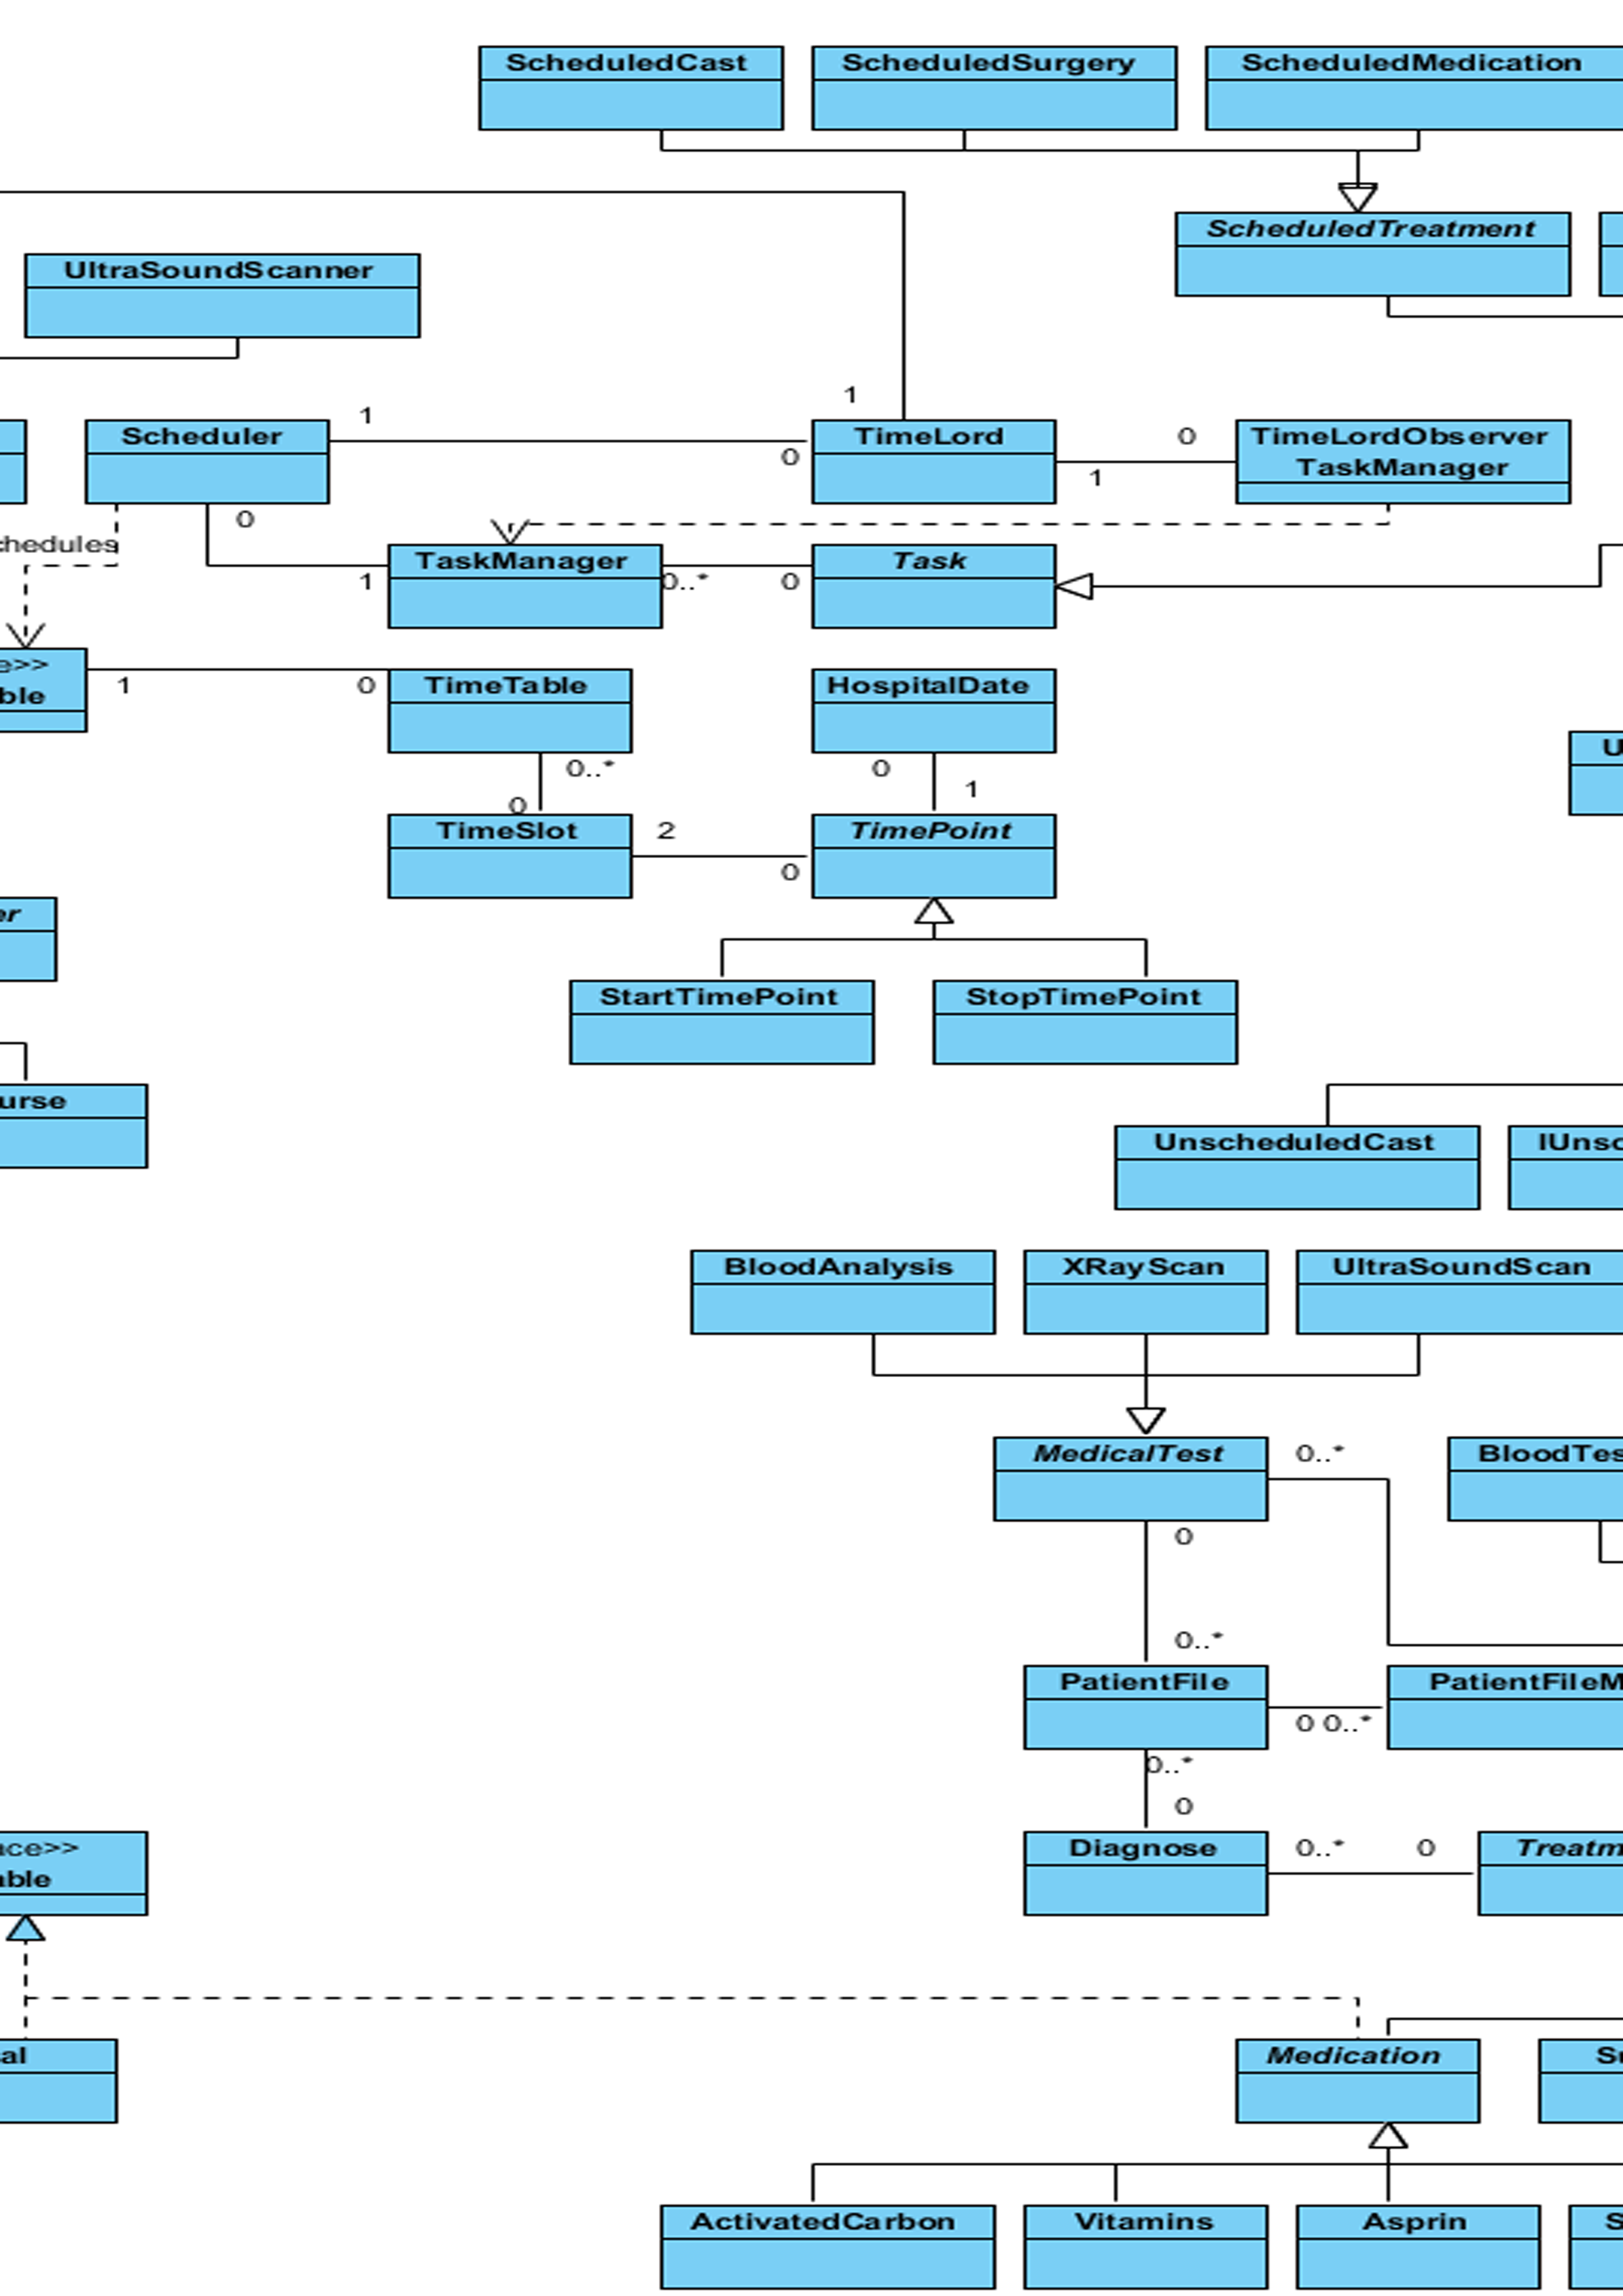
\includegraphics[width=170mm]{left2.png}\\
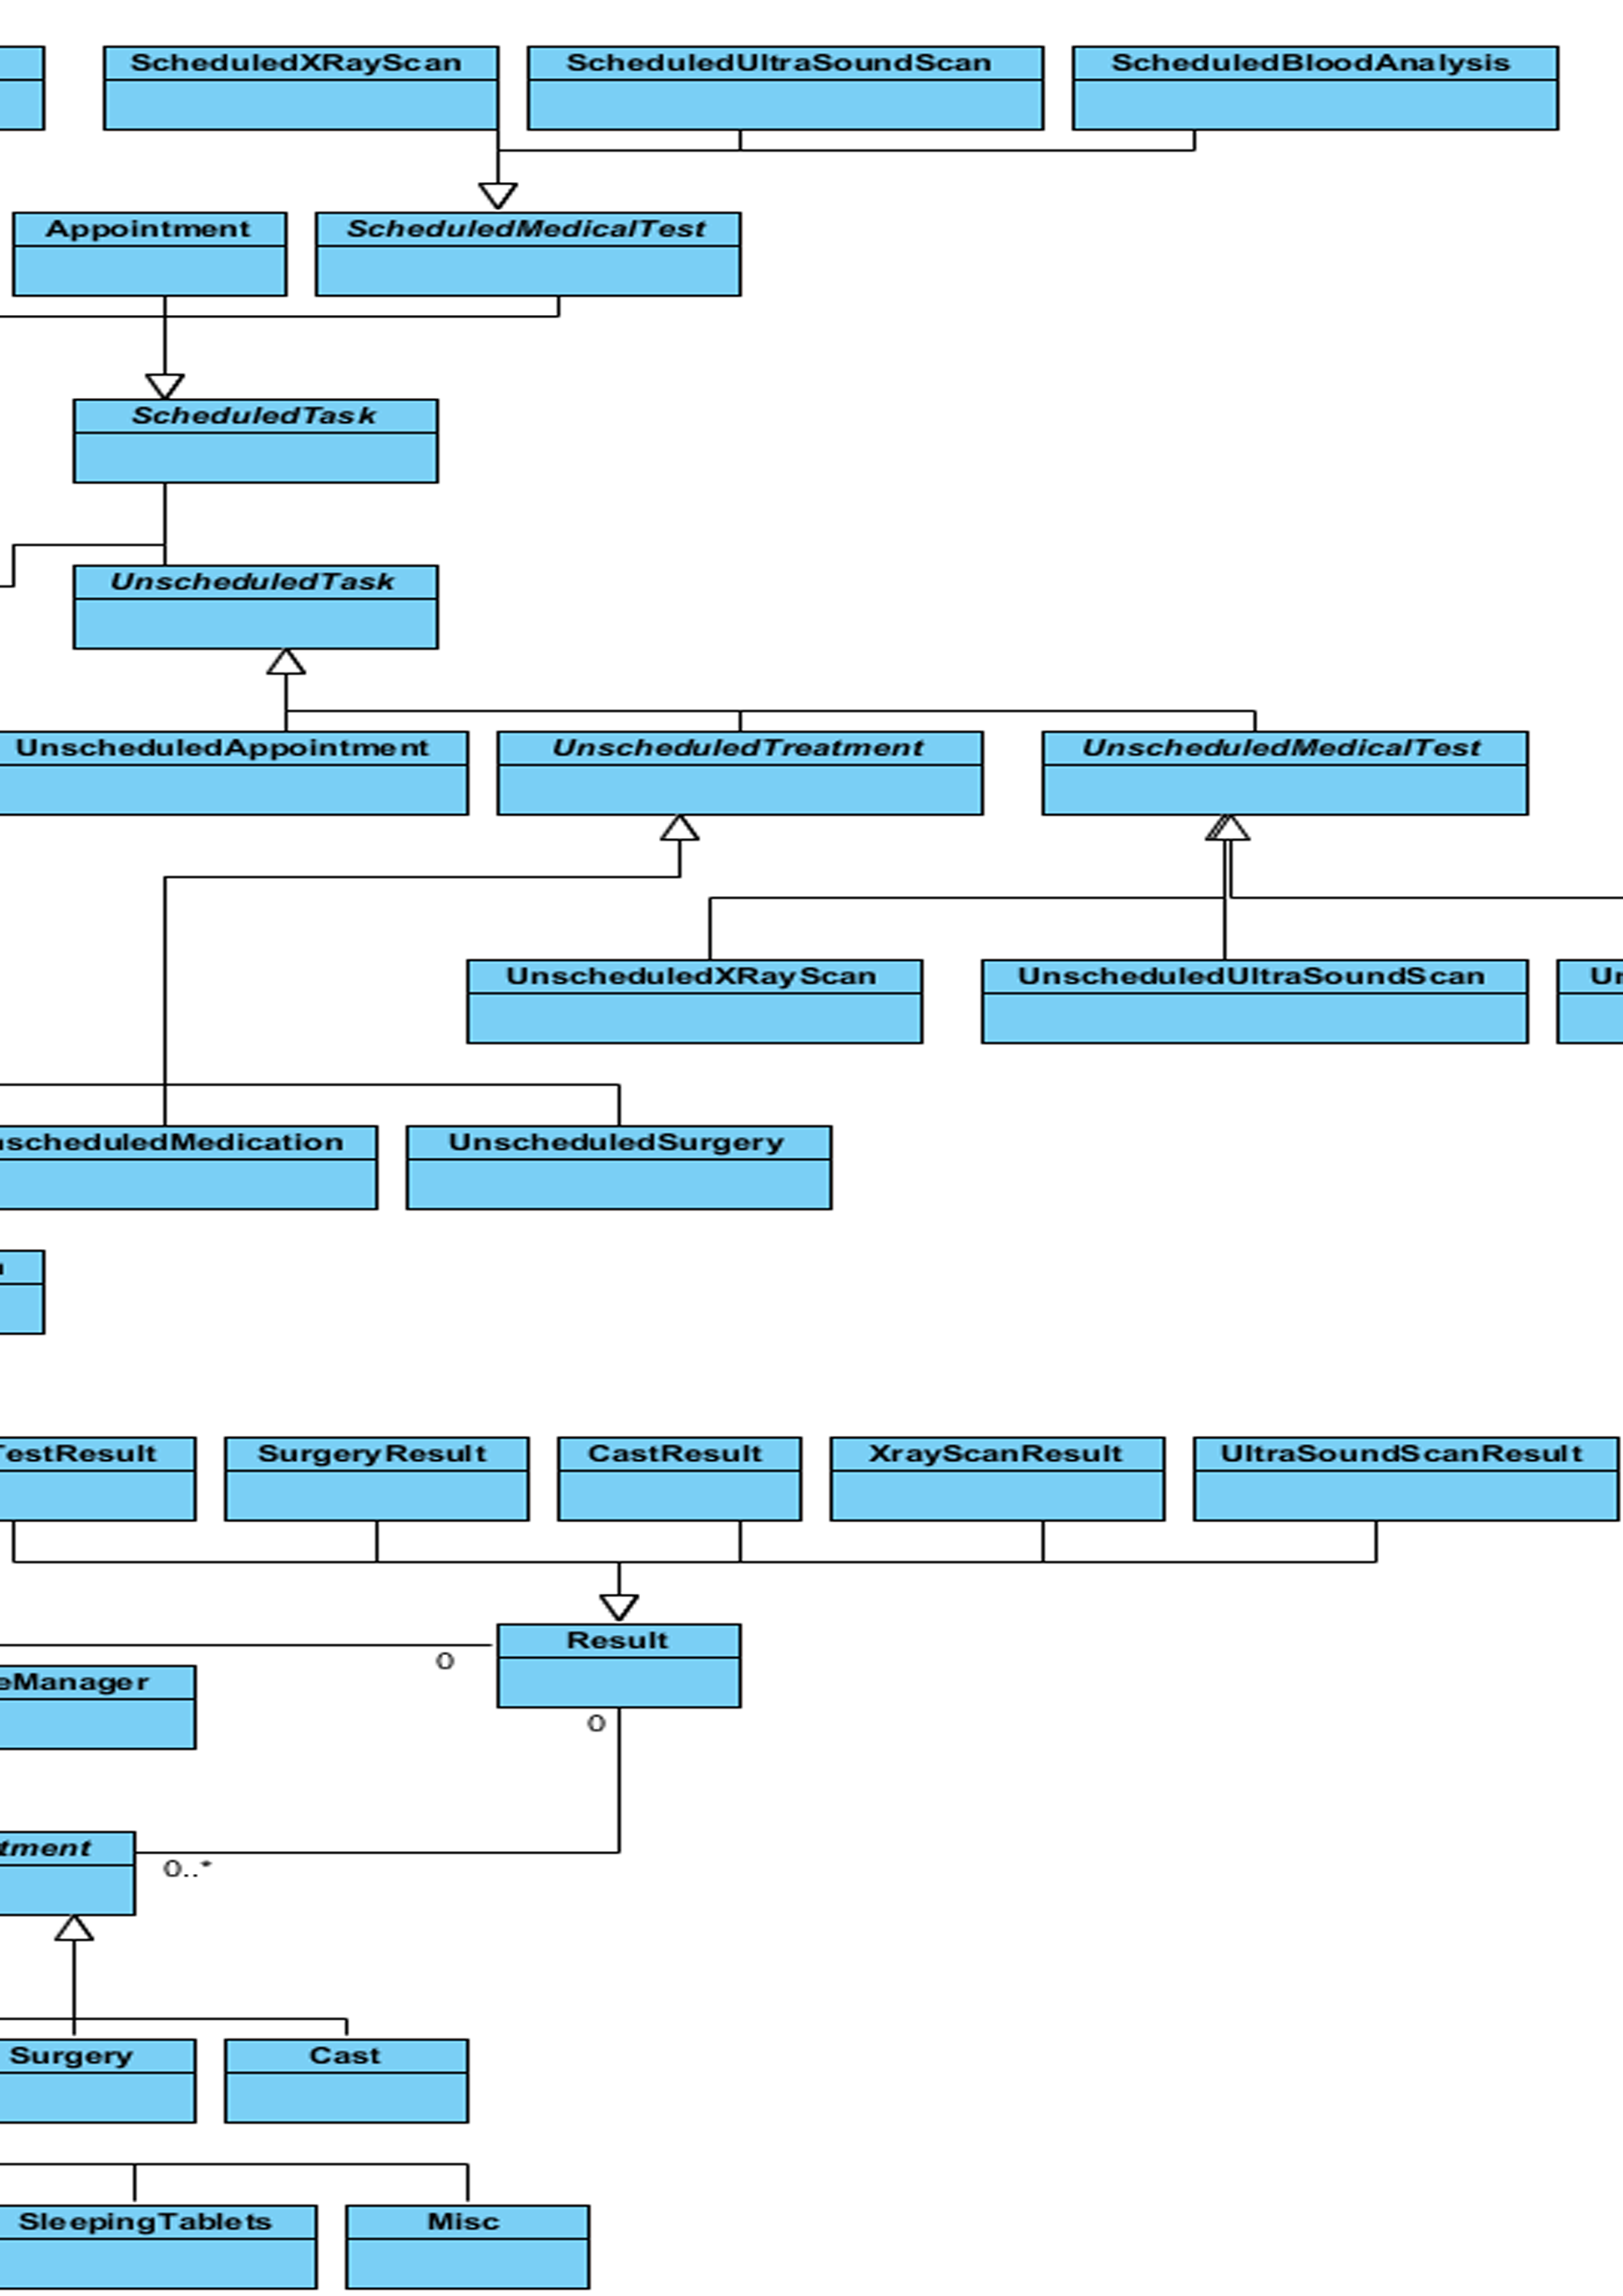
\includegraphics[width=170mm]{middle.png}\\
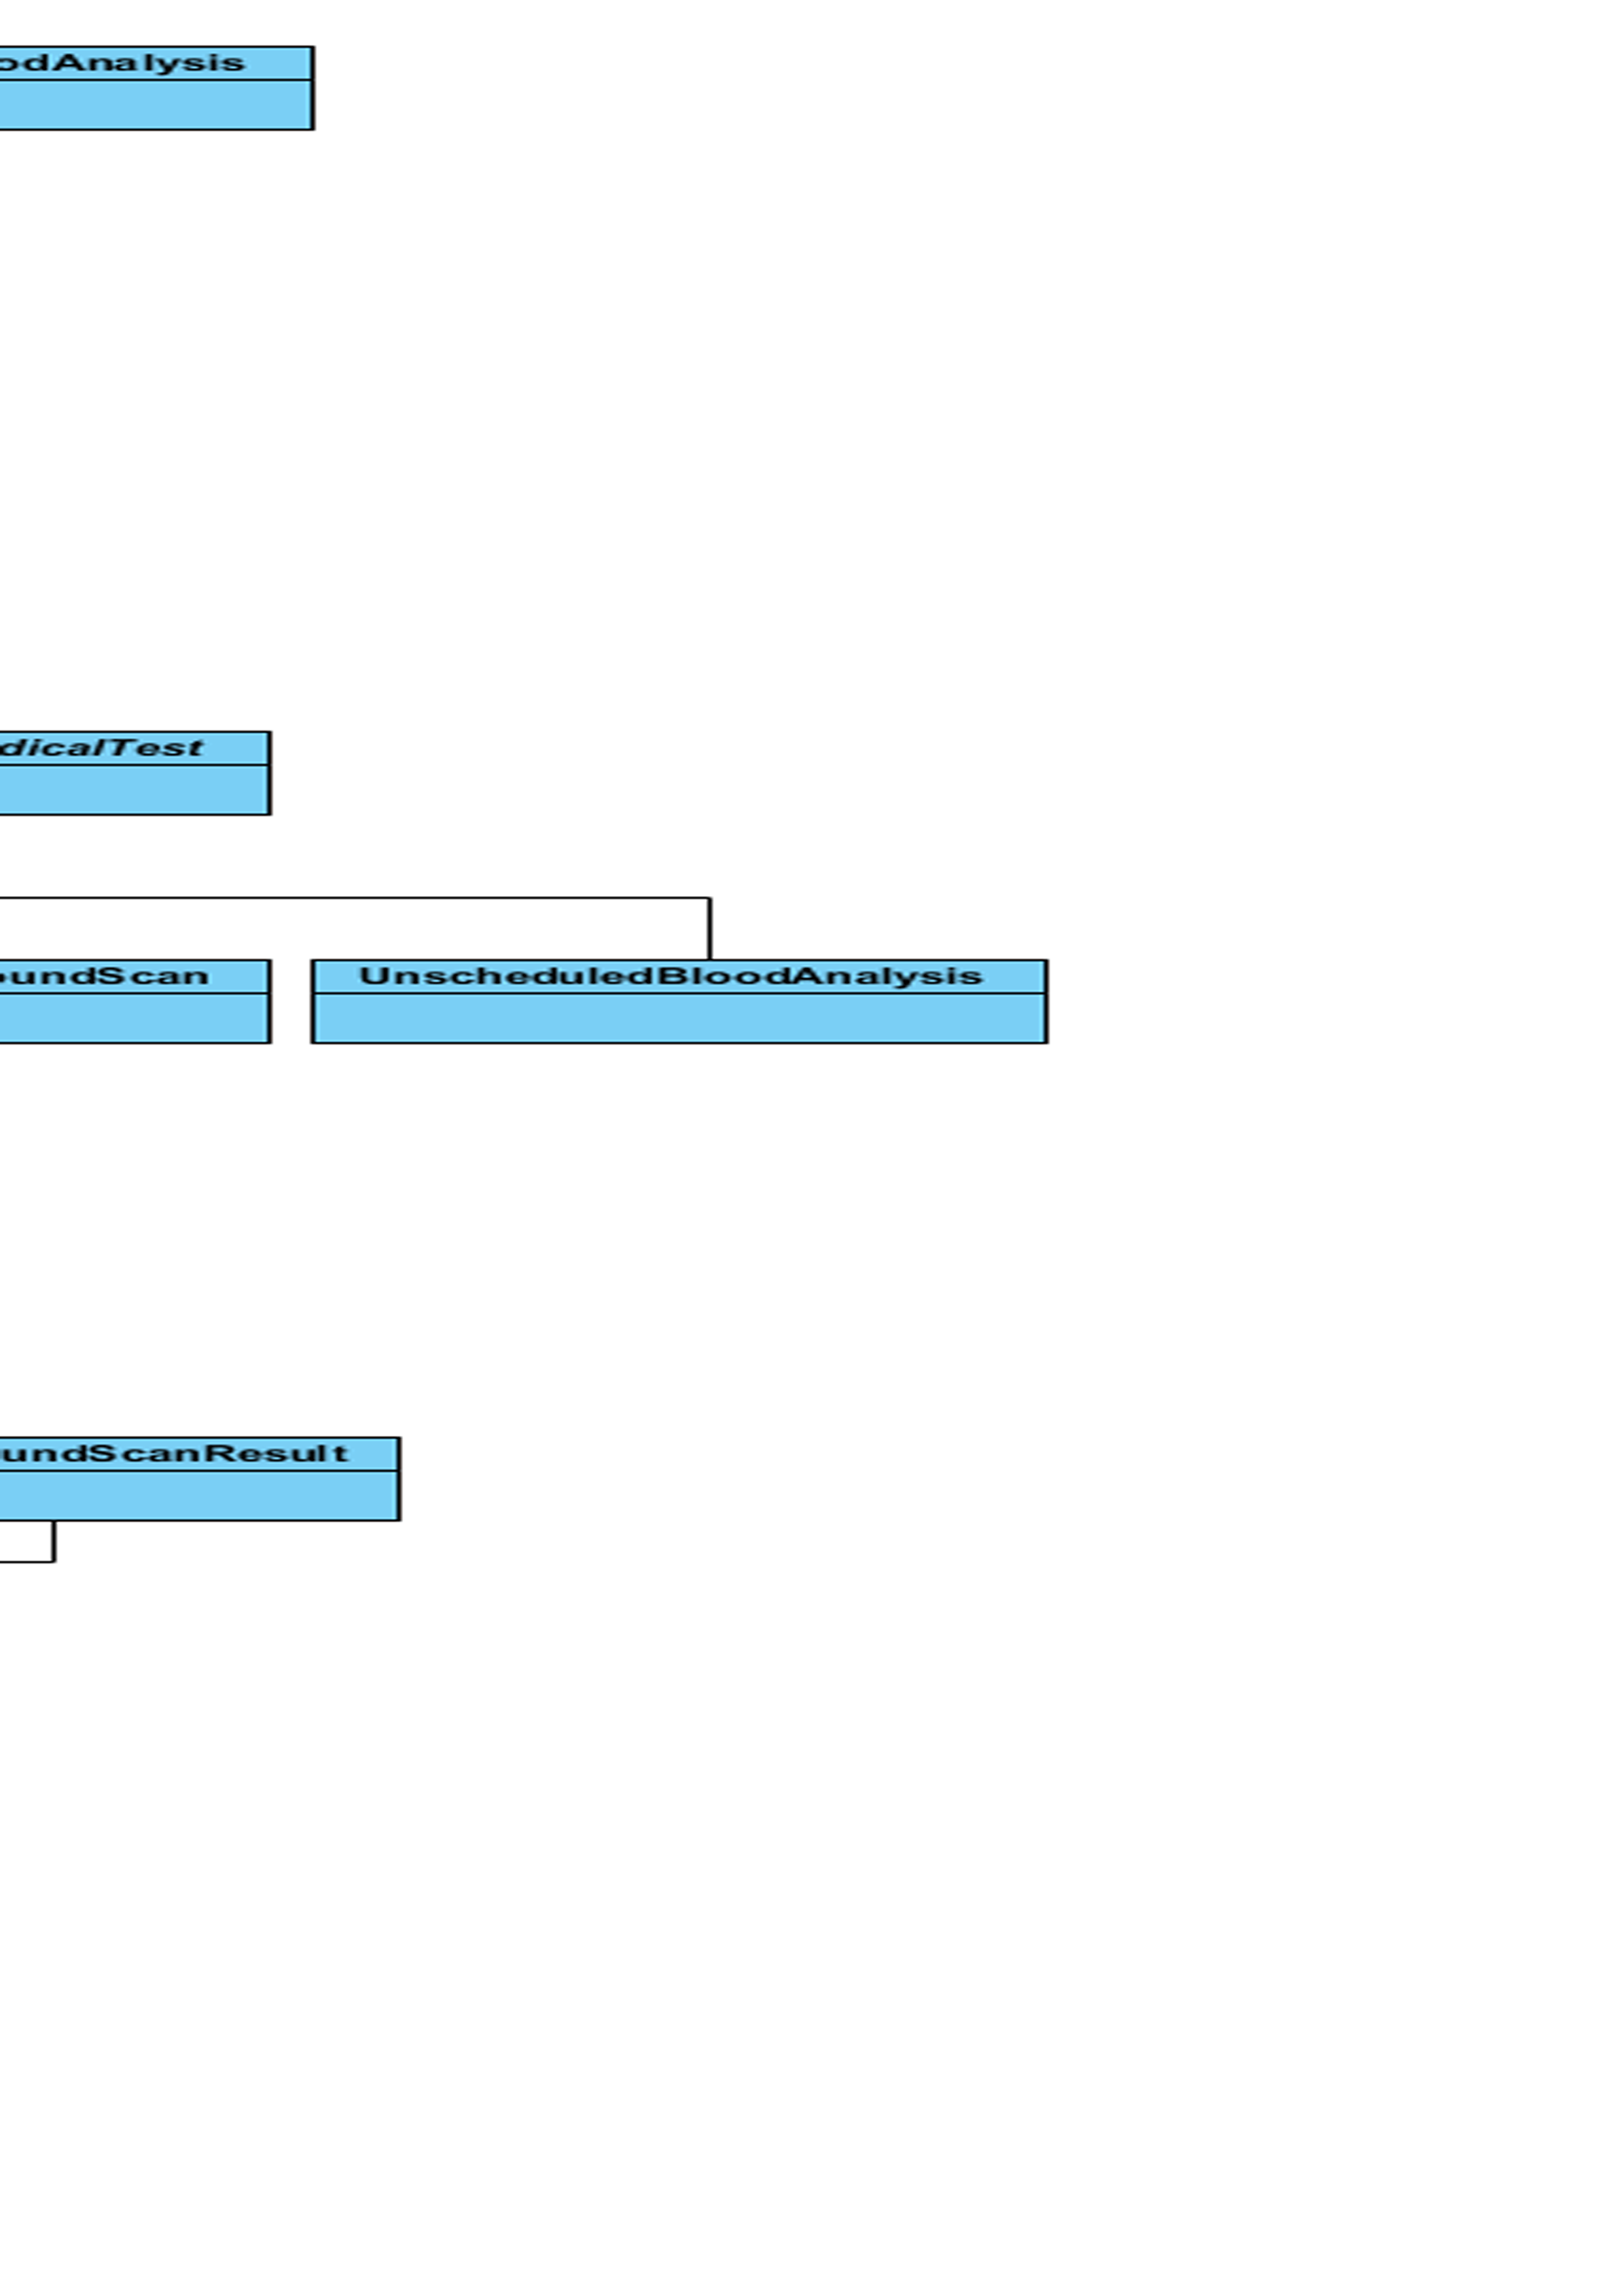
\includegraphics[width=170mm]{right.png}\\


\subsection{MedicalTest, Treatment, Machine and Medication}

\subsection{Current version of Scheduler}
\subsubsection{HospitalDate}
\subsubsection{TimeTable}
\subsubsection{TimePoint}
\paragraph{StartTimePoint}
\paragraph{StopTimePoint}
\subsubsection{TimeSlot}
\subsubsection{Schedulable}
\subsubsection{Constraints}
\subsubsection{Task, UnscheduledTask, ScheduledTask, TaskManager}
\subsection{Alternatives and older versions of Scheduler}
\subsubsection{Original version}
\subsubsection{First revision}
\subsubsection{Second revision}
\section{Use cases}
\section{Other relevant changes}
\subsection{Domain protection - not leaking internal data structures}
\subsection{Defensive programming}
\section{Testing and code coverage}
\section{Conclusion and outro}

\end{document}